%
\documentclass[a4paper,12pt,twoside]{article}
\usepackage{iftex}

%% Разрешить компиляцию только с движком LuaTex
\ifLuaTeX
\else
    \newlinechar 64\relax
    \errorcontextlines -1\relax
    \immediate\write20{@
        ************************************************@
        * LuaLaTex is required to compile this document.@
        * Sorry!@
        ************************************************}%
    \batchmode\read -1 to \@tempa
\fi

%% Для русификации достаточно подключить пакет fontspec и
%% выбрать Unicode шрифт в котором есть кириллические глифы. Ниже
%% основным шрифтом выбирается Unicode версия шрифта Computer Modern с заcечками
\usepackage{fontspec}
\setmainfont{CMU Serif}
\setsansfont{CMU Sans Serif}
\setmonofont{CMU Typewriter Text}

%% В XeLaTex или LuaLaTeX альтернативой известного пакета babel является пакет polyglossia.
%% Теперь у нас будут переносы слов
\usepackage{polyglossia}
\setdefaultlanguage{russian}
\setotherlanguage{english}

\usepackage[autostyle]{csquotes} % Правильные кавычки в зависимости от языка
\usepackage{totcount}
\usepackage{setspace}

% ToDo:
% [] MathNote   : \sum[] syntax
% [] MathNote   : \tikzmatrix 
% [] Layout     : A4 geometry
% [] Layout     : Define colors
% [] References : Load knowledge
% [] References : Create simple clever refs
% [] Fix hidding enviroment

%Отключить предупреждения об кастномной использовании пакетов "You have requested package..."
\usepackage{silence}
\WarningFilter{latex}{You have requested package}

\usepackage{xparse}
\usepackage{configuration/floats}
\usepackage{configuration/layout}
\usepackage{configuration/references}
\usepackage{configuration/mathnote}

\sloppy
% Окружения для набора задач
\newcounter{boxlblcounter}  

\newcommand{\task}[1]{\fbox{\begin{minipage}{4em}\centering\it #1\end{minipage}}}
\newcommand{\makeboxlabel}[1]{\fbox{\begin{minipage}{2em}\centering\it #1\end{minipage}}\hfill}% \hfill fills the label box
\newenvironment{tasklist}
  {\begin{list}
    {\arabic{boxlblcounter}}
    {\usecounter{boxlblcounter}
     \setlength{\labelwidth}{3em}
     \setlength{\labelsep}{0em}
     \setlength{\itemsep}{2pt}
     \setlength{\leftmargin}{1.5cm}
     \setlength{\rightmargin}{2cm}
     \setlength{\itemindent}{0em} 
     \let\makelabel=\makeboxlabel
    }
  }{\end{list}}


\newboolean{ShowHint}
\newboolean{ShowSolution}

% Подсказка
\newcommand{\hint}[1]{\ifthenelse{\boolean{ShowHint}}{\noindent\rotatebox[origin=c]{180}{\noindent
\begin{minipage}[t]{\linewidth} \noindent \it Указание: #1 \end{minipage}}}{}}

% solution: окружение для набора решений
% solution*: форсировано показывает решение, независимо от флага
\makeatletter
\newenvironment{solution*}[1][\text{Решение}]{ 
  \par
  \pushQED{\qed}%
  \normalfont
  \topsep0pt \partopsep3pt
  \trivlist
  \item[\hskip\labelsep
    \itshape
    #1\@addpunct{.}]\ignorespaces
}{
  \ifthenelse{\boolean{ShowSolution}}{
    \popQED\endtrivlist\@endpefalse
    \addvspace{6pt plus 6pt} % some space after
  }{\end{hidden}}
}
\makeatother

%https://tex.stackexchange.com/questions/533218/hiding-an-environment-that-contains-minted-code
%https://tex.stackexchange.com/questions/38150/in-lualatex-how-do-i-pass-the-content-of-an-environment-to-lua-verbatim
\RequirePackage{luacode}
\begin{luacode*}
do 
    function eat_buffer(buf)
        i,j = string.find(buf,"\\end{solution}")
        if i==nil then return "" else return nil end
    end
    function start_proccesing_solution(eat)
        if eat then luatexbase.add_to_callback('process_input_buffer', eat_buffer, 'eat_buffer') end
    end
    function stop_proccesing_solution(eat)
        if eat then luatexbase.remove_from_callback('process_input_buffer', 'eat_buffer') end
    end
end
\end{luacode*}
%https://tex.stackexchange.com/questions/537219/conditionals-inside-newcommand-with-empty-argument
%https://tex.stackexchange.com/questions/63223/xparse-empty-arguments
\ExplSyntaxOn
\DeclareExpandableDocumentCommand{\IfNoValueOrEmptyTF}{mmm}{\IfNoValueTF{#1}{#2}{\tl_if_empty:nTF {#1} {#2} {#3}}}
\NewDocumentCommand{\DefaultName}{mm}{\IfNoValueOrEmptyTF{#1}{#2}{#1}}
\ExplSyntaxOff

% WARNING!
% Buggy: one have always have
% \begin{solution}{NAME}
%   ....
% \end{solution}
% EVEN if NAME is empty
% if one starts some text on the same line as \begin{solution} or \end{solution} it could'not be hidden
\newenvironment{solution}[1]%
{
  \ifthenelse{\boolean{ShowSolution}}
    {\begin{solution*}[\DefaultName{#1}{\textit{Решение}}]\directlua{flag_eat=false}}
    {\directlua{flag_eat=true}}
  \directlua{start_proccesing_solution(flag_eat)}
}
{
  \ifthenelse{\boolean{ShowSolution}}{\end{solution*}}{}
  \directlua{stop_proccesing_solution(flag_eat)}
}


\newcommand{\PracticeSubject}{}
\newcommand{\PracticeName}{}
\newcommand{\PracticeGroup}{}
\newcommand{\PracticeCourse}{}
\newcommand{\PracticeDate}{}


\AtBeginDocument{%
    % Метаданные:
    \title{\PracticeName}%
    \date{\PracticeDate}%
    % Настраиваем колонтитулы
    \pagestyle{fancy}%
    \lhead{\PracticeGroup, курс \PracticeCourse}%
    \chead{\PracticeSubject. Практика}%
    \rhead{\PracticeDate}%

    % Название практики
    \section*{\strtitle}
}
\mmzset{memo dir = images/cache/\jobname}


\setboolean{ShowHint}{false}
\setboolean{ShowSolution}{true}

\renewcommand{\PracticeSubject}{Дискретная математика}
\renewcommand{\PracticeName}{Функции, множества и счётность}
\renewcommand{\PracticeGroup}{ПАДИИ}
\renewcommand{\PracticeCourse}{1}
\renewcommand{\PracticeDate}{23 января 2025}


\begin{document}
\begin{?}
    Пусть множества $A$ и $B$ равномощны. Докажите, что множества $A \times A$ и $B \times B$ также равномощны.
\end{?}
\begin{solution}{}
    Так как $A$ и $B$  равномощны, существует биекция $f  \colon A \to B$. Нетрудно видеть, что отображение:
    \begin{align*}
        & f \times f \colon A \times A \to B \times B \\
        & (a_1, a_2) \mapsto (f(a_1), f(a_2))
    \end{align*}
    также является биекцией так как у любого элемента $(b_1, b_2)$ есть прообраз, причем этот прообраз единственен и равен $(f^{-1}(b_1), f^{-1}(b_2))$.
\end{solution}
\begin{?}
    Докажите, что множество простых чисел счетно.
\end{?}
\begin{solution}{}
    Пусть $\mathbb P \subset \N$ --- множество всех простых чисел. Положим:
    $$
        \mathfrak{p}(n) = \min\set{p \in \mathbb P | n < p}
    $$ 
    Иными словами $\mathfrak{p}(n)$ --- наименьшее простое число превосходящее $n$. В силу бесконечности множества простых чисел, для любого натурального $n$ найдетеся простое число его превосходящее. Не трудно также понять что среди всех таких чисел можно выбрать минимальное. Поэтому $\mathfrak{p}(n)$ корректно определено для всех $n \in \N$. Теперь рассмотрим отображение:
    $$
        n \mapsto \underbrace{\mathfrak{p}\mleft(\mathfrak{p}\mleft(\ldots \mathfrak{p}(2) \ldots \mright)\mright)}_{n-1 \text{ раз}} = \mathrm{prime}(n)
    $$
    Понятно что $\mathrm{prime}(n)$ инъективно, так $\mathrm{prime}(i) <  \mathrm{prime}(j)$  если $i < j$, поэтому у любого простого числа есть не более одного прообраза. Покажем что для всякого простого числа $p_0 \in \mathbb P$ при этом найдется такое натуральное число $n_0$ что $p_0 =  \mathrm{prime}(n_0)$. Предположим противное, т.е. что не все простые числа попали в образ отображения $\mathrm{prime}(n)$. Говоря простым языком, предположим что не все простые числа были занумерованы. Рассмотрим наименьшее из незанумерованных простых чисел, и обозначим его $p_0$. Положим также:
    $$
        p' = \max\set{p \in \mathbb P | p \leq p_0}
    $$
    По предположению, все простые числа меньшие $p_0$ были занумерованы, в том числе было и $p'$, т.е $p' = \mathrm{prime}(n')$ для некоторого $n' \in \N$. Тогда, по определению $\mathrm{prime}$ и $\mathfrak{p}$:
    $$
        \mathrm{prime}(n' + 1) = \mathfrak{p}\mleft(\mathrm{prime}(n')\mright) = \mathfrak{p}(p') = p_0
    $$
    Но это противоречит тому что $p_0$ незанумеровано. Противоречие, и значит $\mathrm{prime}$ устанавлиет биекцию между множеством простых чисел и множеством натуральных.


    \textit{Комментарий для придирчивых.} Это решение достаточно аккуратное, однако существует и более простое решение. Раз $\mathbb{P} \subset \N$ (очевидно) и $\mathbb{P}$ бесконечно, то $\mathbb{P}$ имеет мощность не больше чем мощность натуральных чисел. Но мощность натуральных чисел (счетность) это наименьшая бесконечная мощность, которую может иметь множество. Это вполне хорошое решение. Однако, проблема заключается в том что последнее утверждение требует доказательтсва, которое вовсе не очевидно и степень его тривиальности зависит от определения "бесконечного множества"\,. Подробно можно прочитать \href{https://math.stackexchange.com/questions/1618121/the-smallest-infinity-and-the-axiom-of-choice}{здесь}. К тому же, если принебречь одной из аксиом теории множеств (а именно аксиомой выбора), вполне может статься что будут существовать неэквивалентные определения бесконечного множества: детали см. \href{https://math.stackexchange.com/questions/688708/example-of-a-set-that-is-dedekind-finite-but-not-tarski-finite}{здесь}. 
\end{solution}


\begin{?}
    Докажите, что множество конечных подмножеств рациональных чисел счетно.
\end{?}
\begin{solution}{}
    Обозначим $\mathcal{P}_{\mathrm{fintie}}(\Q)$ множество конечных подмножеств рациональных. Его элементами например являются такие множества:
    $$
        \set{\tfrac{1}{2}}, \set{\tfrac{5}{3}, \tfrac{3}{4}},  \set{\tfrac{1}{2}, \tfrac{5}{3}, \tfrac{3}{4}}  
    $$
    Для начала, пусть $\mathcal{P}_k(\Q)$ это все $k$-элементные подмножества $\Q$ и $\mathcal{P}_k(\N)$. Покажем что $\mathcal{P}_k(\Q)$ можно занумеровать. Так как нам известно, что существует биекция $r : \Q \to \N$, то легко определяется биекция:
    \begin{align*}
        & r_k \colon \mathcal{P}_k(\Q) \to \mathcal{P}_k(\N) \\
        & \set{q_1, \ldots, q_k} \mapsto \set{r(q_1), \ldots, r(q_k)}
    \end{align*}
    Поэтому достаточно построить нумерацию $\mathcal{P}_k(\N)$. Это легко сделать. Сначала рассмотрим случай $k = 2$, общая конструкция строится аналогично, но описание становится более громоздким. В случае $k = 2$, мы можем записать:
    $$
        \mathcal{P}_k(\N) = \set{\set{i, j} \subset \N | i, j \in \N, i \neq j} = \set{(i, j), i, j \in \N | j < i}
    $$
    понимая каждое двухэлементное подмножество $\N$ как упорядоченную пару, где на первом месте стоит больший элемент, а на втором месте младший. Понятно что такое  множество легко занумеровать:
    \begin{figure}[h!]
        \centering
        \includetikz{practice-01-solution-img-01.tikz}
    \end{figure}
    
    \noindent Аналогичную нумерацию можно построить при любом $k$. Итак, мы получили биекцию
    \begin{align*}
        & f_k \colon \mathcal{P}_k(\Q) \to \N \\
        & \set{q_1, \ldots, q_k} \mapsto n_{q_1, \ldots, q_k}
    \end{align*}
    Наконец построим биекцию между 
    $$
        f_{\mathrm{finite}} \colon \mathcal{P}_{\mathrm{fintie}}(\Q) = \bigcup_{k = 1}^{\infty}\mathcal{P}_k(\Q) \to \N \times \N
    $$
    А именно, определим:
    $$
        f_{\mathrm{finite}}(\set{q_1, \ldots, q_k}) = (f_k(\set{q_1, \ldots, q_k}), k)
    $$
    Таким образом, $k$-элементному множеству сопоставляется его номер при нумерации $f_k$ и собственно число элементов в нем. Это биекция, так как по размеру множества и его номеру в соответствующей нумерации множество однозначно восстанавливается. Более того любая пара $(n, k)$ отвечает какому-то подмножеству. Но $\N \times \N$ равномощно $\N$, поэтому и $\mathcal{P}_{\mathrm{finite}}(\Q)$ равномощно $\N$.
\end{solution}
\begin{?}
    Установите взаимно однозначное соответствие между множеством бесконечных последовательностей из 0 и 1 и множеством бесконечных последовательностей из
    \begin{itemize}[noitemsep, topsep=0pt, parsep=3pt]
        \item  0, 1, 2, 3;
        \item 0, 1, 2.
    \end{itemize}
\end{?}
\begin{solution}{}
    В первом случае просто будем использовать двоичное кодирование по два бита:
    \begin{align*}
        & 0 \mapsto 00 \quad 1 \mapsto 01 \\
        & 2 \mapsto 10 \quad 3 \mapsto 11
    \end{align*}
    Получится примерно такое соответствие:
    $$
        \underbrace{00}_{0}\underbrace{01}_{1}\underbrace{01}_{1}\underbrace{10}_{2}\underbrace{11}_{1} \ldots.
    $$
    Чтобы установить соответствие между множеством последовательностей из 0,1 и множеством последовательностей из 0,1,2, нам потребуется чуть более хитрая конструкция.
    $$
        0 \mapsto 1 \quad 1 \mapsto 01 \quad 2 \mapsto 00
    $$
    Тогда понятно что любая последовательность из $0,1,2$ переводится в какую-то последовательность из $0, 1$. Но верно и обратное, так как мы можем просто декодировать слева направо:
    $$
        \underbrace{1}_{0} \underbrace{01}_1 \underbrace{00}_2 \underbrace{01}_1 \underbrace{1}_0 \underbrace{00}_2
    $$
\end{solution}
\begin{?}
    Установите взаимно-однозначное соответствие между
    \begin{itemize}[noitemsep, topsep=0pt, parsep=3pt]
        \item Сферой без точки и плоскостью;
        \item Между интервалом $(0, 1)$ и прямой $(-\infty, +\infty)$;
        \item Между $\R$ и $\R^2$;
        \item Между $[0; 1]$ и $2^{\mathbb{N}}$
    \end{itemize}
\end{?}
\begin{solution}{}
    \begin{itemize}[noitemsep, topsep=0pt, parsep=3pt]
        \item Используем так называемую стереографическую проекцию. См. рисунок:
        \begin{figure}[h]
            \centering
            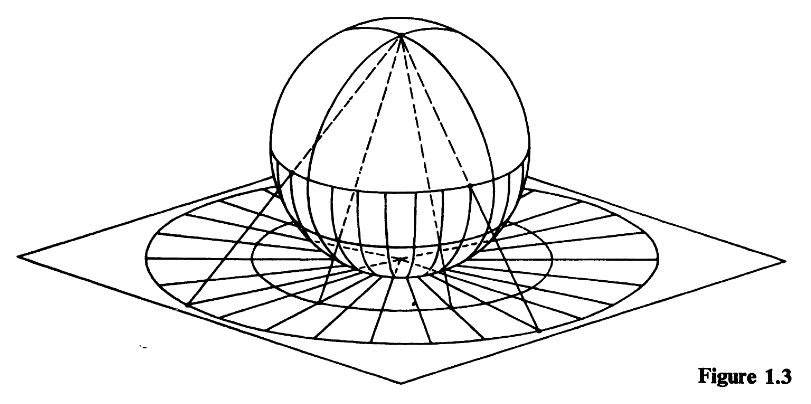
\includegraphics{practice-01-solution-img-02}
        \end{figure}

        \item Между интервалом $(0, 1)$ и прямой $(-\infty, +\infty)$ можно дать биекцию:
        $$
            y = \tan\mleft(\frac{\pi}{2}(x+1)\mright)
        $$
        \item Между $\R$ и $\R^2$ биекцию можно построить следующим образом: понятно что есть следующие биекции:
        \begin{align*}
            & \R \to (0; 1) \\
            & \R^2 \to (0; 1) \times (0; 1)
        \end{align*}
        Просто в силу предыдущего пункта и первой задачи. Поэтому будем строить биекцию между $(0;1)$ и $(0;1)\times(0;1)$. Это можно сделать например следующим образом: возьмем десятичную запись произвольного числа:
        $$
            0.b_1b_2b_3\ldots
        $$
        И цифры на четных позициях сопоставим первому числу в паре, а цифры в нечетных позициях --- второму.
        $$
            0.b_1b_2b_3\ldots \mapsto (0.b_2b_4b_6\ldots, 0.b_1b_3b_5\ldots)
        $$
        \textit{Комментарий для придирчивых}. Тут возникает тонкий вопрос, связанный с тем что некоторые десятичные числа можно записывать двумя способами:
        $$
            0.4999\ldots = 0.5000\ldots 
        $$
        Однако на самом деле десятичными записями вещественных чисел и самими вещественными числами можно построить биекцию. Это верно потому что чисел, которые имеют более чем одну запись будет всего лишь счетное число, и каждое такое число имеет ровно две не совпадающие записи. Также, то что мы сделали это формально биекция между $[0; 1]$ и $[0; 1] \times [0; 1]$, но в домашнем задании будет задача в которой вы докажете что между $(0; 1)$ и $[0; 1]$ есть биекция. 

        \item Между $[0; 1]$ и $2^{\mathbb{N}}$. Это задача похожа на предыдущую. Действительно, каждое число из $[0; 1]$ можно представить в виде своей двоичной записи:
        $$
            0.101010010 
        $$
        Ему можно сопоставить бинарную последовательность, получаемую отсечением строки $0.$, и тогда мы получаем просто бинарную строку. Чтобы предъявить биекцию с множеством всех подмножеств натуральных чисел, рассмотрим такое правило:
        $$
            b_1 \ldots b_k \ldots \mapsto \set{i \in \N | b_i = 1}
        $$ 
        Иными словами каждой бинарной строке мы сопоставляем множество позиций, в которых стоит цифра 1. Нетрудно проверить что это биекция.
    \end{itemize}
\end{solution}
\begin{?}
    Докажите, что только бесконечное множество может быть равномощно собственному подмножеству.
\end{?}
\begin{solution}{}
    Пусть $A$ конечно, $B \subsetneq A$ его подмножество и $|B| = |A|$. Но так как $B \subsetneq A$, то множество $A \setminus B$ не пусто и значит $|A \setminus B| > 0$. При этом, так как все множество конечны:
    $$
        |A| = |B| + |A \setminus B|
    $$
    С другой стороны по предположению $|B| = |A|$, и значит $|A \setminus B| = 0$, противоречие.
\end{solution}
\end{document}

